% !TEX encoding = UTF-8
% !TEX TS-program = pdflatex
% !TEX root = ../tesi.tex

%**************************************************************
\chapter{Protocolli di modellazione e trasferimento dati}
\label{cap:protocolli-trasmissione-dati}
%**************************************************************

\intro{Nel seguento capitolo vengono trattati dal punto di vista teorico i protocolli di modellazione e trasferimento dati, in particolare viene approfondito lo stile architetturale REST e il linguaggio di query GraphQL.
}\\

%**************************************************************
\section{Introduzione ai protocolli}
\subsection*{Modello architetturale client-server}
\label{client-server}
Prima di procedere nella spiegazione sui protocolli di trasferimento e modellazione dati, è necessario fare una breve introduzione sull'architettura delle Web Application moderne. Queste seguono ormai tutte un modello server - client, ovvero un modello architetturale che divide in due processi l'applicazione: un client che richiede servizi al server, il quale li esegue ritornando una risposta contenente l'esito dell'operazione. I protocolli di trasferimento e modellazione dati trovano il loro maggior utilizzo proprio nella comunicazione client - server, tuttavia prima di procedere con la loro spiegazione è necessario introdurre il concetto di Application Programming Interfaces.
\subsection*{Application Programming Interfaces}
 Comunemente dette API, ovvero l'acronimo di Application Programming Interfaces, sono interfacce comunemente realizzate per aggevolare la comunicazione tra  server e client. Ciascun applicativo/dispositivo è sviluppato con strutture di dati differenti che evolvono nel tempo, dunque risulta complessa la comunicazione tra queste entità. Le API giocano un ruolo fondamentale nello scambio di dati: infatti definiscono una interfaccia per la comunicazione, la quale è indipendente dall'implementazione specifica del dispositivo o dell'applicativo e permette di comunicare secondo delle regole specifiche riportate nella propria documentazione. Risultano dunque fondamentali nella comunicazione, collaborazione e integrazione di nuovi componenti applicativi.\\ \\
 Al giorno d'oggi le API vengono utilizzate dalla maggior parte delle web applications, dispositivi IoT, applicativi di vario genere e molto altro ancora.
 Nello specifico nella tesi si fa riferimento alle Web API, ovvero a quelle interfacce che sfruttano il protocollo HTTP per la comunicazione con altri applicativi/dispositivi. Ci sono diversi tipi di Web API, tra queste:
 \begin{itemize}
   \item \textbf{API pubbliche}: si tratta di API accessibili da tutti (possono essere anche a pagamento);
   \item \textbf{API private}: si tratta di API create con lo scopo di essere utilizzate solo ed esclusivamente all'interno dell'azienda;
   \item \textbf{API partner}: si tratta di API utilizzate tra aziende in collaborazione;
   \item \textbf{API composte}: si tratta di API differenti combinate tra loro per creare una sequenza di operazioni.
 \end{itemize}
La necessità di standardizzare il modo in cui vengono sviluppate le interfacce API ha portato dunque alla nascita dei protocolli sul trasporto di dati.
\subsection*{Protocolli di trasferimento dati}
Per protocolli di modellazione e trasferimento dati s'intende un insieme di regole, strutture e vincoli che regolano il funzionamento delle API. Permettono dunque di definire una sorta di standard al quale gli sviluppatori possono far riferimento per implementare e interagire con le API. Il termine protocollo non si addice perfettamente a tutte le varie tecnologie di data fetching, tuttavia a grandi linee può racchiuderle e dunque verrà utilizzato per questione di comodità.
\subsection*{I primi protocolli e loro evoluzione}
Al giorno d'oggi il protocollo di modellazione e trasferimento dati più utilizzato è sicuramente REST, tuttavia sono presenti anche altre tipologie di protocolli in utilizzo o che comunque sono state utilizzate in passato. Si tratta di tecnologie con lo stesso scopo, ma di natura completamente differente, di seguito le principali.
\subsubsection*{Remote Procedure Call}
Viene spesso indicato con l'acronimo RPC, si tratta di protocollo secondo il quale una procedura o subroutine viene invocata da un client esterno al server che deve eseguire la procedura, senza che il client conosca i dettagli del network. Viene utilizzato per chiamare processi in sistemi remoti, ma come fossero locali. \\
Di seguito riportata la definizione attribuita all'RPC dagli informatici Andrew Birrell e Bruce Nelson nel 1984:
  \begin{quoting}
    “Meccanismo sincrono che trasferisce il flusso di controllo e i dati attraverso una chiamata di procedura tra due spazi di indirizzo su una rete a banda stretta.”
  \end{quoting}
Come nelle chiamate a procedure locali, un RPC è una operazione sincrona che tiene in pausa il client fino al momento in cui ritorna il risultato della procedura invocata.
\subsubsection*{Simple Object Access Protocol}
Indicato spesso con l'acronimo SOAP, si tratta di un vero e proprio protocollo che definisce la struttura dei dati che devono essere trasferiti e come questi devono essere elaborati. Richiede esclusivamente il formato XML per trasferire dati e tipicamente viene utilizzato il protocollo HTTP per il trasferimento di file, tuttavia possono essere utilizzati anche protocolli differenti come ad esempio il protocollo SMTP. La struttura di un messaggio SOAP è composta da 3 principali componenti:
\begin{itemize}
  \item \textbf{Envelope}: necessario al fine di identificare il documento come messaggio SOAP;
  \item \textbf{Header}: è opzionale. Lo scopo dell'header nei messaggi SOAP è quello di trasportare indicazioni estranee al messaggio che si vuole trasportare, ma che vengono interpretate da i diversi nodi durante il cammino del messaggio;
  \item \textbf{Body}: il body contiene il vero e proprio messaggio che si vuole trasferire.
\end{itemize}
\subsubsection*{Ad hoc}
\section{Approfondimento sullo stile architetturale REST}
REST è l'acronimo di "Representational State Transfer" e si tratta di un tipo di stile architetturale introdotto da Roy Fielding nel 2000 e viene considerato al giorno d'oggi come uno standard per la realizzazione di web API. Si tratta di una astrazione degli elementi di un architettura di un sistema, del quale REST ne ignora i dettagli del'implementazione delle componenti e della sintassi del protocollo imponendo dei vincoli sul loro ruolo e sulla loro interazione.
\subsection*{Principi di un architettura REST}
\label{principi-REST}
Un architettura REST dunque deve rispettare alcuni principi, di seguito verranno elencati i sei gruppi definiti da Fielding.
\subsubsection*{Client-server}
Il primo principio sposa uno dei paradigmi cardine dell'informatica, ovvero il principio di \textit{Separation of concerns}, secondo il quale conviene sempre separare un sistema complesso in moduli distinti in modo che ognuno possa avere un proprio compito.\\
Ciò viene ripreso nell'architettura REST separando il client dal server, dunque dividendo due logiche diverse in due moduli distinti. Così facendo server e client possono essere implementati in maniera indipendente, usando qualsiasi lingua o tecnologia, basta che siano conformi al prossimo principio detto \textit{uniform interface}.
\subsubsection*{Uniform interface}
Si tratta di un principio fondamentale che differenzia le REST API da qualsiasi API non REST. Secondo questo prinpicio l'interazione tra componenti Web, dunque client, server e tutti gli intermediari del network, dipendono dalla uniformità delle loro interfacce.\\
I componenti Web dunque sono in grado di comunicare coerentemente seguendo quattro vincoli sull'interfaccia delineati da Fielding; questi sono:
\begin{itemize}
  \item \textbf{Identification of resources}: le risorse che vengono richieste devono essere identificate nella richiesta stessa, dunque specificandole nell'url;
  \item \textbf{Manipulation of resources through representations}: il client deve avere la rappresentazione delle risorse e deve poter sapere come modellarle sul server. L'idea alla base è che la rappresentazione (attraverso un qualsiasi formato, ad es. JSON, XML, ecc...) è una modo per interagire con le risorse, ma non è la risorsa stessa;
  \item \textbf{Self-descriptive messages}: in ciascun messaggio devono esser presenti le informazioni necessarie a descrivere come deve essere processata la richiesta;
  \item \textbf{Hypermedia as the Engine of Application State}: la rappresentazione dello stato di una risorsa deve includere i riferimenti alle risorse correlate. É dunque necessario includere i link per ciascuna risposta, così che il client possa navigare tra le altre risorse facilmente.
\end{itemize}
\subsubsection*{Layered System}
Secondo questo principio l'architettura di un applicativo deve essere composta da più strati. Ciascuno strato inoltre è cieco rispetto agli altri strati, tranne per quanto riguarda gli strati adiacenti. Questi layer possono essere composti da intermediari basati sul network i quali intercettano la comunicazione client-server con uno scopo specifico (ad esempio per questioni di sicurezza, caching, controllo del flusso dati, ecc...), possono essere ad esempio proxy e gateways. Per il principio di Layered System questi intermediari devono aderire alle interfacce al fine di mantenerne l'uniformità.
\subsection*{Cache}
Si tratta di uno dei vincoli fondamentali in un archiettura Web, secondo il quale un web server deve dichiarare la \textit{cacheability} di ciascuna risposta ritornata. Più specificatamente qualsiasi risposta di un server deve etichettare come cacheabili o meno i dati presenti all'interno di esso. Così facendo gli intermediari tra server e client e il client stesso sanno come comportarsi riguardo alla memorizzazione dei dati.
\subsection*{Stateless}
Il vincolo di stateless fa riferimento al fatto che un server non deve memorizzare lo stato dell'applicazione client. Questo implica però che ogni richiesta che il server riceve dal client deve essere sufficientemente dettagliata sullo stato del client affinché il server sia in grado di eseguirla. Dunque le richieste non sono correlate tra loro e per questo viene definito "stateless". \\
Questo vincolo porta un vantaggio fondamentale secondo il quale un server così facendo può gestire richieste da molti client. Può inoltre esser scalato molto più facilmente con l'aiuto ad esempio di un load balancer.
\subsection*{Code on demand}
Per ultimo troviamo il vincolo di code on demand, si tratta di un vincolo facoltativo secondo il quale la logica del client può essere aggiornata indipendentemente da quella lato server. Un esempio pratico lo troviamo nella signel web application le quali rispettano totalmente queste vincolo.

\section{Approfondimento sul linguaggio di query GraphQL}
\subsection*{Introduzione}
GraphQL è stato ideato da Facebook nel 2012 e condiviso e reso pubblico nel 2014. Al giorno d'oggi molte importanti applicazioni  utilizzano GraphQL, come ad esempio GitHub, Twitter, PayPal e Pinterest. Viene considerato come il principale competitor e possibile successore di REST nell'ambito del data fetching, tuttavia come verrà spiegato in seguito, oltre a svariati punti di forza e di innovazione ha anche alcuni problemi.\\
Più nello specifico GraphQL è un linguaggio di query per le APIs. Viene definito agnostico rispetto al mezzo di trasporto perché non dipende dal modo in cui client e server comunicano, ma solitamente viene utilizzato sul protocollo HTTP. Il principale punto di forza di GraphQL è la possibilità di specificare nella query esattamente i dati che si è interessati a ricevere, questo permette dunque di non occupare la rete per dati non richiesti. Altro importante punto di forza, ma che talvolta può risultare un problema, è che è fortemente tipizzato.\\
Affermare che GraphQL abbia lo scopo di servire esclusivamente come linguaggio di query può risultare riduttivo. Una dei principali motivi d'utilizzo di GraphQL è quello di riuscire a raggruppare tutti i dati e servizi di un'applicazione insieme in uno stesso posto, e fornire così un'interfaccia unica che risulti consistente, sicura e infine semplice da utilizzare.\\
GraphQL non specifica come deve essere costruita un'API, tuttavia ci sono cinque linee guida dette "Principi di desing" da tenere in considerazione durante lo sviluppo di un API:
\begin{itemize}
  \item \textbf{Hierarchical}: i tipi ricercati in una query GraphQL seguono una struttura gerarchica, infatti i tipi possono avere come campi altri tipi e così via. Inoltre i dati che vengono ritornati dalla query, vengono ritornati esattamente con la medesima struttura con cui sono stati richiesti;
  \item \textbf{Product centric}: le API sono inevitabilmente guidate dalle richieste dal client, per questo bisogna realizzarle in maniera flessibile cercando di tener conto delle richieste client per permettere quanto richiesto;
  \item \textbf{Strong typing}: un server GraphQL è supportato da un type system specifico a seconda dell'applicazione. Data una query, il server assicura che questa sia sintatticamente corretta, valida e che i tipi in gioco rispettino esattamente la struttura dei tipi definiti nel GraphQL schema;
  \item \textbf{Client-specified queries}: in GraphQL, la codifica della query avviene nel client e non nel server e si tratta di query che vanno a specificare campo per campo. Nella maggiorparte dei sistemi che non utilizzano GraphQL, il server determina quali dati ritornare. In GraphQL ciò non accade, vengono infatti ritornati solo i dati specificati dal client;
  \item \textbf{Introspective}: GraphQL è introspettivo, infatti i clients possono consultare a fondo il GraphQL schema e possono dunque vedere tutte le query disponibili, i vari tipi e i loro campi.
\end{itemize}
\subsection*{GraphQL schema}
GraphQL ha cambiato il modo di pensare alle APIs: queste non vengono più considerate come un insieme di endpoints dai quali ottenere dati ed eseguire servizi, ma vengono piuttosto considerate come una collezione di tipi.\\
La progettazione delle APIs GraphQL risulta essere differente da come avviene negli altri protocolli, infatti prima di procedere con l'implementazione delle APIs, è necessario definire i tipi di dati che verranno esposti e richiesti dalle APIs. Questo approcio viene denominato "\textbf{Schema first}" e si tratta di una tecnica che prevede appunto come prima fase della progettazione del sistema di APIs, la creazione di una sorta di pagina nella quale radunare tutti i tipi necessari, questo posto viene definito \textbf{GraphQL Schema}. È importante definire nel dettaglio all'interno dello schema tutti i tipi che possono essere richiesti e inviati dai clients. Così facendo poi gli sviluppatori frontend saranno in grado di conoscere nel dettaglio la struttura di ciascun tipo e delle varie query. Le APIs sviluppate con GraphQL si autodocumentano proprio perché è sufficiente la consultazione dello schema per comprendere la natura delle entità che si desidera interrogare o modellare.\\
\subsection*{Definizione dei tipi}
Come detto in precedenza la caratteristica principale di GraphQL è che si tratta di un linguaggio di query fortemente tipizzato. I tipi sono l'unità principale di un GraphQL schema.\\
Per tipo s'intende un oggetto costruito dettagliatamente campo per campo che deve poi corrispondere ad una entità nel backend dell'applicativo. Dunque all'interno dello schema dovranno essere definiti tutti i tipi che andranno a rappresentare la struttura dati dell'applicativo.\\
Un tipo può contenere come campi dati altri tipi che sono definiti nel medesimo schema. Segue un esempio di tipo dichiarato in uno schema GraphQL, in questo caso si tratta della dichiarazione di un Employee:
\begin{verbatim}
  type Employee {
    id: ID
    name: String!
    owns: Badge
    worksIn: Department
    worksOn: [Project]
    ...
  }
\end{verbatim}
In questo caso il tipo Employee avrà come campi:
\begin{itemize}
  \item \textbf{id}: un codice identificativo di tipo \textit{ID};
  \item \textbf{name}: un nome di tipo \textit{String}, il punto esclamativo indica che si tratta di un campo che non può essere nullo;
  \item \textbf{owns}: un badge di tipo \textit{Badge} per l'accesso al dipartimento;
  \item \textbf{worksIn}: un dipartimento di tipo \textit{Department} nel quale lavora l'impiegato,
  \item \textbf{worksOn}: una lista di progetti di tipo \textit{Project} al quale l'impiegato sta lavorando.
\end{itemize}
I tipi \textit{Department}, \textit{Badge} e \textit{Project} dovranno essere necessariamente definiti all'interno dello stesso GraphQL schema di Employee;
I built-in type che GraphQL mette a disposizione vengono detti \textbf{scalar type} e sono: \textit{Int}, \textit{String}, \textit{Boolean}, \textit{ID}, \textit{Float}.
È possibile inoltre dichiarare anche degli scalar type personalizzati con la keywork "\textit{scalar}", oppure delle enumerazioni attraverso l'utilizzo della keyword "\textit{enum}". È possibile infine unire diversi tipi, molto utile nel caso in cui si volesse ritornare uno tipo tra un insieme di tipi, questo è possibile farlo con la keyword "\textit{union}" come segue:
\begin{verbatim}
  union worker = Employee | Manager | Chief
\end{verbatim}
In questo caso sono stati uniti in un unico tipo \textit{worker} i tipi \textit{Employee}, \textit{Manager} e infine \textit{Chief}. Verrà molto utilizzato successivamente il tipo unione nella gestione degli errori di ritorno al client dopo l'esecuzione delle query.
\subsection*{Connessioni tra tipi}
GraphQL è cosi denominato perché oltre ad essere un Query Language come suggeriscono le ultime due lettere del nome, permette di definire connessioni di vario genere tra i tipi definiti nello schema, queste connessioni vanno di fatto a creare uno grafo composto da tipi interconnessioni, da questo deriva il prefisso \textit{Graph}.
È fondamentale durante la definizione del GraphQL schema riportare le relazioni nella maniera corretta delle entità corrispondenti nel database dell'applicativo. Un'ultima premessa prima di visualizzare i vari tipi di connessioni riguarda la direzionalità delle connessioni: in GraphQL risulta essere una buona pratica dare bidirezionalità alle connessioni ove possibile, questo con lo scopo di lasciare più flessibilità possibile allo sviluppatore client il quale dalla una query specifica può raggiungere diversi tipi e spostarsi nel grafo come più desidera.\\
Di seguito vengono elencate le varie relazioni con relativi esempi.
\subsubsection*{Connessione one-to-one}
Nelle relazioni one-to-one ad un tipo viene associata una sola istanza di un altro tipo e viceversa. Riprendendo il caso del tipo Employee riportato sopra, possiamo trovare una relazione del tipo one-to-one tra i tipi Employee e Badge. Di seguito la rappresentazione del grafo:
\begin{figure}[!h]
\centering
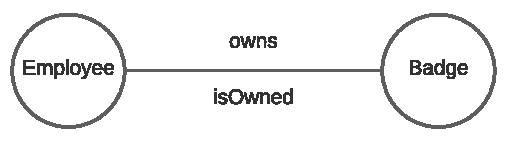
\includegraphics[width=0.5\linewidth]{immagini/one_to_one.pdf}
\caption{Connessione one-to-one.}
\label{one-to-one}
\end{figure}
\\ \\
Come mostrato in figura \ref{one-to-one} il collegamento tra i due tipi è definito come "owns" se si legge nel verso che parte da Employee per raggiungere Badge e fa riferimento all'omonimo campo di Employee. Se altrimenti la connessione si percorre nel verso opposto viene definita "isOwned", come l'omonimo campo di Badge, riportato in seguito:
\begin{verbatim}
  type Badge {
    id: ID
    isOwned: Employee
    ...
  }
\end{verbatim}
\subsubsection*{Connessione one-to-many}
In questo caso bisogna focalizzarsi sul campo \textit{worksIn} di Employee. Questo campo definisce la connessione con un elemento di tipo \textit{Department}, dunque a ciascun impiegato corrisponde un dipartimento nel quale lavora. Tuttavia pensando alla connessione in senso opposto a ciascun dipartimento possono corrispondere più impiegati. Segue dunque la rappresentazione della connessione nel grafo:\\

\begin{figure}[!h]
\centering
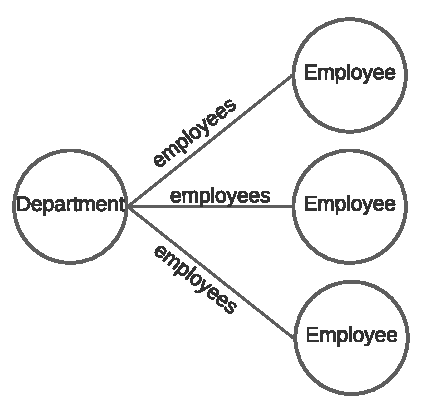
\includegraphics[width=0.4\linewidth]{immagini/one_to_many.pdf}
\caption{Connessione one-to-many.}
\label{one-to-many}
\end{figure}
\mbox{}\\
Come mostrato in figura \ref{one-to-many} il collegamento tra il dipartimento e i vari impiegati viene chiamato "employees" se si considera il verso che parte da Department per raggiungere Employee e corrisponde all'omonimo campo di Department. Tuttavia il collegamento è definito "worksIn" se la connessione viene percorsa nel verso opposto. Segue la rappresentazione del tipo Department:
\begin{verbatim}
  type Department {
    id: ID
    name: String!
    address: String!
    employees: [Employee]
  }
\end{verbatim}
\subsubsection*{Connessione many-to-many}
Consideriamo ora il campo \textit{worksOn} di Employee che collega ciascun impiegato con una lista di progetti ai quali sta lavorando. In questo caso però considerando il collegamento nel verso opposto anche ciascun progetto può avere più impiegati che ci lavorano. In questo caso si tratta di una relazione many-to-many e segue la rappresentazione nel grafo:
\begin{figure}[!h]
\centering
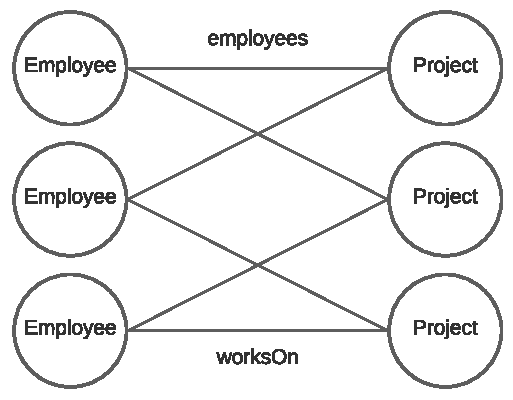
\includegraphics[width=0.4\linewidth]{immagini/many_to_many.pdf}
\caption{Connessione many-to-many.}
\label{many-to-many}
\end{figure}
\\ \\
% da sistemare questi doppi backslash
Le relazioni many-to-many non sono altro che l'unione di due relazioni one-to-many.
La connessione in questo caso, come nei casi precedenti, a seconda del verso in cui viene percorsa può esser definita come "worksOn" o "employees" come mostrato in figura \ref{many-to-many}. Di seguito la rappresentazione del tipo Project:
\begin{verbatim}
  type Project {
    id: ID
    name: String
    employees: [Employee]
  }
\end{verbatim}
\subsection*{Operazioni sui dati}
Come detto in precedenza GraphQL è un linguaggi di query e come tale permette di interrogare i dati o eseguire operazioni su di essi. Ci sono tre tipi di operazioni che possono essere fatte sui dati e queste sono: \textit{Query}, \textit{Mutation} e infine \textit{Subscription}.
\subsubsection{Query}
L'operazione di query viene utilizzata per richiedere dati da una determinata API ed equivale alla GET nel protocollo REST. È necessario dichiarare nel GraphQL schema la query che il programmatore backend desidera rendere disponibile, così facendo vengono dichiarati anche i tipi che possono eventualmente essere passati come argomenti e quelli che verranno ritornati dalla query.\\
Un esempio di dichiarazione di query che ritorna una lista di tutti gli oggetti di tipo Employee presenti in un determinato Department può essere:
\begin{verbatim}
  type query {
    employeesInDepartment(departmentId: ID!): [Employee]
  }
\end{verbatim}
In questo caso invocando la query \textit{employeesInDepartment} e passando come argomento alla query l'id (non può essere un valore nullo) del dipartimento, riceveremo come risposta un JSON contenente un campo "\textit{data}" contenente a sua volta la lista di impiegati, questo se la query ha avuto successo. In caso di insuccesso della query per qualsiasi motivo, ad esempio per avere passato un id errato, allora verrà ritornato un JSON con un campo "\textit{error}", contenente la descrizione dell'errore. \\
Dal punto di vista del client, qualora si volesse invocare questa query bisognerebbe strutturare la richiesta come segue:
\begin{verbatim}
  query {
    employeesInDepartment(id: "2BR4S") {
      id
      name
      worksOn {
        id
        name
      }
    }
  }
\end{verbatim}
Se la query non dovesse fallire, verrà ritornata una lista di impiegati e per ciascun impiegato verranno ritornati i campi specificati nella query dunque: l'\textit{id}, il \textit{name}, una lista di oggetti di tipo Project nel campo \textit{worksOn} per i quali bisognerà a loro volta specificare i campi ai quali si è interessati, in questo caso all' \textit{id} e al \textit{name} di ciascun progetto.\\
È inoltre possibile utilizzare gli argomenti delle query per controllare la quantità di dati che possono esser ritornati con un processo chiamato \textit{data paging}, oppure usarli per decidere in che ordine vogliamo che vengano ritornati i dati.
\subsubsection*{Mutation}
L'operazione di mutation viene utilizzata per eseguire modifiche sui dati. Equivale all'unione delle operazioni POST, DELETE, PUT, PATCH nel protocollo REST. Come per le query è necessario dichiarare le mutation che si voglion rendere disponibili al client.\\
Un esempio di mutation può essere:
\begin{verbatim}
  type mutation {
    addNewEmployee(employee: Employee!): Employee
  }
\end{verbatim}
In questo caso la mutation \textit{addNewEmployee} andrà ad aggiungere un nuovo impiegato nella struttura dati dell'applicativo. Il client per invocare questa mutation dovrà strutturare la richiesta come segue:
\begin{verbatim}
  mutation {
    addNewEmployee(employee: {
      name: "Mario"
    }){
      id
    }
  }
\end{verbatim}
In questa mutation è stato passato come argomento un oggetto di tipo Employee, del quale è stato specificato esclusivamente il nome (va obbligatoriamente specificato essendo un campo dichiarato non nullo). Come da definizione la mutation ritorna un oggetto di tipo Employee, del quale però in questo caso si vuole ricevere solo l'id generato. Come nel caso della query, se l'aggiunta dell'impiegato avrà successo, nel JSON di ritorno ci sarà un campo \textit{data} contenente l'id generato in seguito all' aggiunta dell'impiegato, in caso contrario sarà ritornato un JSON con un campo \textit{error} che descrive l'origine dell'errore.
\subsubsection*{Subscription}
L'ultimo tipo si chiama Subscription e si tratta di una funzione particolare resa disponibile in GraphQL, infatti grazie a questa funzione i client possono sottoscriversi ad una subscription e così facendo sarà il server ad inviare al client i dati richiesti non appena questi sono disponibili, dunque non è più necessario che sia il client a richiedere periodicamente i dati aggiornati.\\
Un esempio di definizione di una Subscription può essere:
\begin{verbatim}
  type subscription {
    newEmployeeAdded: Employee!
  }
\end{verbatim}
Il client che desidera sottoscriversi alla subscription \textit{newEmployeeAdded} dovrà mandare una richiesta strutturata come segue:
\begin{verbatim}
  subscription {
    newEmployeeAdded {
      id
      name
    }
  }
\end{verbatim}
Così facendo il server, appena viene aggiunto un nuovo impiegato, invierà direttamente al client i dati che il client ha specificato nella sottoscrizione, ovvero in questo caso l'\textit{id} e il \textit{name} dell'impiegato.\\
Essendo il server a dover inviare i dati al client e non il client che richiede i dati dal server, non è utilizzabile il protocollo HTTP per la comunicazione server - client, bisogna quindi utilizzare il protocollo WebSocket per aprire un canale di comunicazione a doppia via sopra un socket TCP.\\ \\
